%%%%%%%%%%%%%%%%%%%%%%%%%%%%%%%%%%%%%%%%%%%%%%%%%%%%%%%%%%%%%%%%%%%%%%%%%%%

\documentclass{standalone}

\usepackage{amsmath}
\usepackage{mathptmx}
\usepackage{pgfplots}
\usetikzlibrary{external}
\tikzexternalize{preston-curve}
\pgfplotsset{compat=1.15}

%% IEEE uses Times Roman font, so we'll default to Times.
%% These three commands make up the entire times.sty package.
\renewcommand{\rmdefault}{ptm}
\renewcommand{\ttdefault}{pcr}
\normalfont\selectfont

\begin{document}

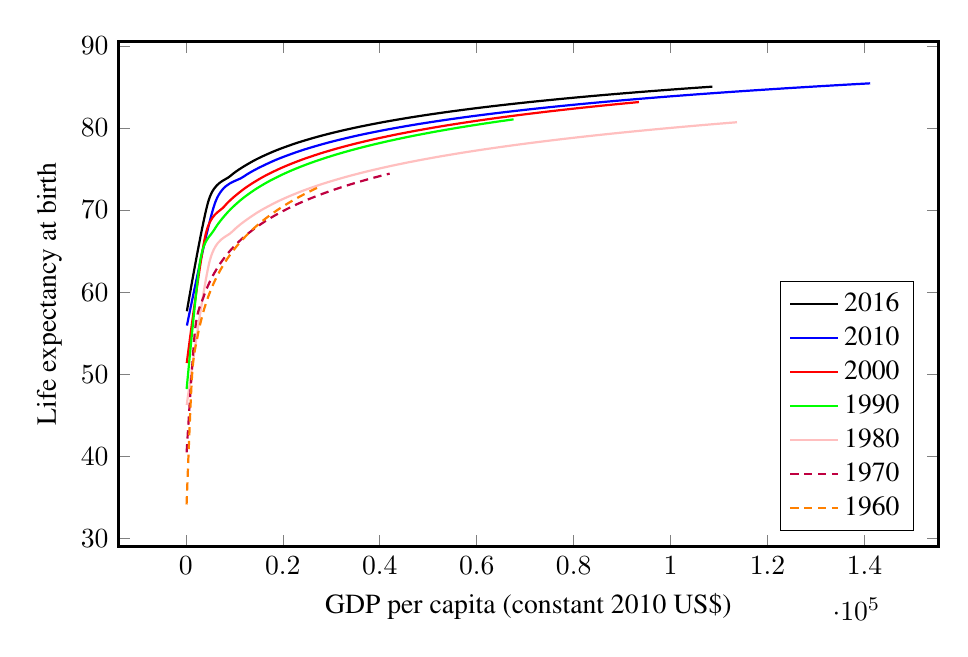
\begin{tikzpicture}
\tikzset{%%
  every mark/.append style={scale=1.0},%%
  scale=1.0%%
}
\pgfplotsset{%%
  every axis/.append style={font=\normalsize}%%
}
%%
\begin{axis}[%%
  axis line style=very thick,%%
  enlargelimits=true,%%
  height=8cm,%%
  legend cell align=left,%%
  legend pos=south east,%%
  plotStyle/.style={%%
    mark=none,%%
    smooth,%%
    thick%%
  },%%
  width=12cm,%%
  %% x axis
  xlabel={\normalsize GDP per capita~(constant 2010 US\$)},%%
  %% y axis
  ylabel={\normalsize Life expectancy at birth}%%
]
%%
%%
\addplot+ [plotStyle,black,domain=218:108601]
{4.4040 * ln(x) + 33.9595};
\addlegendentry{2016}
%%
%%
\addplot+ [plotStyle,blue,domain=231:141166]
{4.5986 * ln(x) + 30.9028};
\addlegendentry{2010}
%%
%%
\addplot+ [plotStyle,red,domain=196:93463]
{5.1534 * ln(x) + 24.1678};
\addlegendentry{2000}
%%
%%
\addplot+ [plotStyle,green,domain=172:67607]
{5.4981 * ln(x) + 19.8960};
\addlegendentry{1990}
%%
%%
\addplot+ [plotStyle,pink,domain=190:113683]
{5.3864 * ln(x) + 17.9890};
\addlegendentry{1980}
%%
%%
\addplot+ [plotStyle,purple,domain=169:42056]
{6.1543 * ln(x) + 8.9141};
\addlegendentry{1970}
%%
%%
\addplot+ [plotStyle,orange,domain=158:27086]
{7.4964 * ln(x) - 3.8128};
\addlegendentry{1960}
\end{axis}
\end{tikzpicture}

\end{document}
